\chapter{Fazit} \label{sec:conclusion}

\section{Evaluation}

Die implementierten Verfahren haben gezeigt, dass mit dem Ansatz der Tiefenbild Überdeckung von \citet{wloka1995resolving} eine Echtzeit Überdeckung virtueller Objekte auf der mobilen Project Tango Hardware erfolgreich umgesetzt werden kann. Dabei wird im Folgenden auf jedes Verfahren sowie ihrer Vor und Nachteile im Kontext der anderen Verfahren und auf Basis der durchgeführten Tests eingegangen. \\

\subsection*{Pointcloud Projektion}

Die Überlagerung durch die Pointcloud Projektion bietet gegenüber den anderen Verfahren den Vorteil, dass sie zu jeder Zeit eine dynamische und aktualisierte Repräsentation der Tiefe der Szene liefert und somit auch Änderungen in der Szene sofort berücksichtigt. Außerdem ist das Verfahren nicht auf Clustergrößen beschränkt und kann dadurch auch auch komplexe Strukturen abbilden. Zu erkennen ist dies bei der Testszene zwei, bei der die Bilddifferenz zum optimalen Ergebnis am geringsten ist, obwohl die Pflanze eine komplexe Struktur besitzt.\\

Dadurch, dass die Pointcloud von Project Tango Fehler in Form von Ausreißern und einem gewissem Rauschen enthalten kann, spiegeln sich diese Fehler auch in der berechneten Projektion wieder. Das führt dazu, dass zum Beispiel die Kante einer realen Überlagerung durchgehend in Bewegung ist und Ihre Struktur mit jedem neuen Tiefenbild variiert. Ein weiteres Problem dieser Technik ist, dass sie, dadurch dass sie sich nur auf einen Datensatz pro Aufnahme bezieht, die Tiefe nur innerhalb des Messbereichs des Tiefensensors repräsentieren kann. Dadurch können Überlagerungen von realen Objekten innerhalb der ersten 50 Zentimeter und ab vier Metern nicht mehr bestimmt werden.\\

\subsection*{Ebenen Rekonstruktion}

Die Ebenen Rekonstruktion löst die Schwächen der Pointcloud Projektion in dem Sinne, dass sie die Ungenauigkeit der Tiefeninformation als eine Oberflächen Approximation mit Hilfe von RANSAC in Form von Ebenen abbildet. Hierdurch werden Ausreißer ignoriert und auch das Rauschen wird durch eine lineare Regression gemittelt. Zusätzlich ermöglicht das Vorgehen der Ebenen Rekonstruktion eine kontinuierliche Verbesserung, indem alle bereits aufgenommenen Pointclouds in die aktuelle Rekonstruktion einfließen. Auch wenn dieser Rekonstruktionsansatz durch den Octree eine Rekonstruktion in einer groben Struktur, den Clustern des Octrees, durchführt, erhält das Verfahren durch das Ermitteln der konvexen Hülle pro gefundener Ebene einen gewissen Detailgrad, um auch schwierige planare Strukturen abbilden zu können. Die gemessenen Ergebnisse der Szenen eins und zwei spiegeln diese positive Eigenschaft wieder und zeigen, dass diese Art der Rekonstruktion auch komplexe Szenen für dieses Testszenario gut abbilden kann.\\

In einem manuellen dynamischeren Test mit Bewegungen weißt dieses Verfahren jedoch einige Schwächen auf. So sind durch die begrenzte Dichte der Pointcloud Lücken zwischen den Ebenen zu sehen, die zwar von Aufnahme zu Aufnahme kleiner werden aber üblicherweise nicht komplett schließen. Das führt dazu, dass zum Beispiel große Oberflächen, die ein virtuelles Objekt überlagern, das Objekt vereinzelt nicht aussparen, da keine Tiefe an den Stellen durch Lücken zwischen den Ebenen vorhanden sind. Außerdem ist das Verfahren nur bedingt in der Lage runde Strukturen wie den Sitzball aus Szene eins zu rekonstruieren. Diese Fehler werden besonders dann sichtbar, wenn man sich um diesen Ball dreht und er eine Überlagerung mit den Ecken und Kanten der Ebenen aus der Rekonstruktion auf ein virtuelles Objekt ausübt. Neben der fehlenden Unterstützung für runde Konturen besitzt dieses Verfahren keine Möglichkeit, Messungen zu revidieren wenn reale Objekte in der Szene verändert wurden oder ein Drift Fehler von Project Tango auftritt.

\subsection*{TSDF Rekonstruktion}

Wie zu erwarten liefert Chisel als eine TSDF Implementierung, aufgrund der großen Voxelgröße, nicht die Qualität, die zum Beispiel ein KinectFusion liefern kann. Dafür ist es performant genug, um als eine CPU Implementierung eine Echtzeit Rekonstruktion auf der mobilen Project Tango Hardware zu ermöglichen. Genau wie die Ebenen Rekonstruktion bietet Chisel den Vorteil eine Rekonstruktion pro Tiefenbild anzureichern und stetig zu verbessern. Dadurch können Überlagerungen auch außerhalb des Messbereichs des Tiefensensors ermöglicht werden. Anders als bei der Ebenen Rekonstruktion generiert die TSDF Rekonstruktion stets eine geschlossene Oberfläche. Außerdem können runde Strukturen festgehalten werden, wodurch der in Szene eins stehende Sitzball abgebildet werden kann. \\

Die große Voxelgöße führt jedoch dazu, dass wie in beiden getesteten Szenen zu erkennen, die Strukturen der Rekonstrutkion sehr grob ausfallen und die Differenzergebnisse ohne eine Filterung auf einen hohen Fehler hinweisen. Auch wenn Chisel nicht in der Lage ist so detailierte Kantenabbildungen wie die Ebenen Rekonstruktion zu generieren, besitzt Chisel einen Vorteil: Durch den Space Carving Mechanismus können Rekonstruktionen wieder revidiert werden. Das hilft dabei den Problematiken des Drift Effekts von Project Tango entgegenzuwirken. Außerdem könnte durch eine GPU Implementierung auch eine Echtzeit Rekonstruktion mit deutlich kleinerer Voxelgröße und dadurch höherem Detailgrad realisiert werden.


\subsection*{Guided Filter}

Der Guided Filter war in den Tests häufig in der Lage selbst grobe Fehler im Tiefenbild an die Kanten der Farbbilder anzugleichen und somit auch, wie in den Messergebnissen zu erkennen, den Differenzwert zum Optimum zu reduzieren. Jedoch führte der Einsatz des Filters zu deutlichen Performanceeinbußen, denn der Filterprozess selbst benötigt im Durchschnitt \(220\) ms. Der Einsatz von OpenCV erschwert zudem den Einsatz des Filters für die Echtzeit Umsetzung, da die Bildebene pro Bild aus dem OpenGL Framebuffer raus und wieder rein geladen werden muss. Dieser Prozess benötigt zusätzliche \(80\) ms, was die Wiederholrate der prototypischen Implementierung auf 3 Herz reduziert. \\

Zusätzlich sind unter gewissen Umständen, bei denen ein virtuelles Objekt nah an der Oberfläche eines realen Objekts, aber immer noch räumlich hinter dem realen Objekt liegt, variable Artefakte aufgefallen, an denen das eigentlich überlagerte virtuelle Objekt durchschimmert. Dieser Effekt ist in Abbildung \ref{fig:artifacts} zu erkennen. Neben den eigentlichen Kanten für die Überlagerung im Farbbildes werden auch Kanten von flachen Strukturen berücksichtigt. Im Bild zu sehen, beeinflusst das Muster vom Würfel das resultierende Tiefenbild soweit, dass eine fehlerhafter Überlagerung nach der Filterung stattfindet. \\
 
\begin{figure}[h]
  \centering
	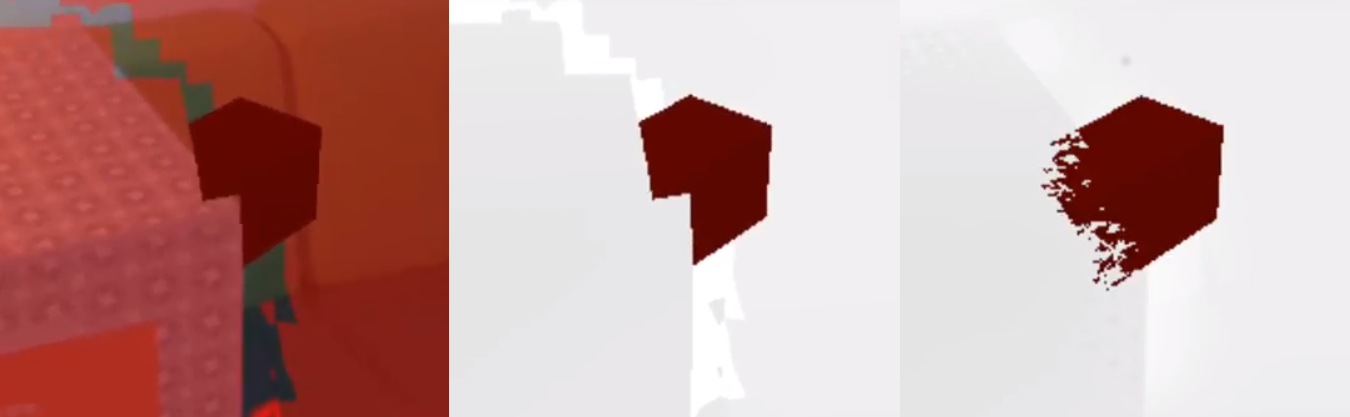
\includegraphics[width=1.0\textwidth]{content/images/artifacts.png} 
  \caption{Fehlerhafte Überdeckung bei der Anwendung des Guided Filters. Links: Reales Objekt mit Rekonstruktion. Mitte: Tiefenbild. Rechts: Sichtbare Fehler nach Guided Filter.}
  \label{fig:artifacts}
\end{figure}

Angewendet auf die Tiefeninformationen der Pointcloud Projektion konnte der Filter in der komplexeren zweiten Szene nahezu das Optimum der Überlagerung erreichen. Schwieriger war jedoch der Einsatz bei der runden Kontur in der ersten Szene, wo der Filter nicht in der Lage war, den initialen groben Fehler vom Tiefensensor zu revidieren. Das selbe Verhalten ist auch bei der Ebenen Rekonstruktion in Szene eins zu beobachten. Besonders beachtenswert ist die Tatsache, dass bei den zu weit reichenden Tiefeninformationen der TSDF Rekonstruktion, in der Mitte der Messergebnisse von Szene eins, ein etwa gleichgroßer Fehler durch die Filterung behoben werden konnte. Eine weitere Besonderheit, die während der Tests beobachtet werden konnte, ist dass der Filter in der Lage war bei der Anwendung auf die Ebenen Rekonstruktion, die Lücken zwischen den Ebenen unkenntlich zu machen. Somit würde dieser Filter ein Nachteil dieses Ansatzes lösen.\\

\section{Einsatz der Verfahren}

Grundsätzlich ist festzuhalten, dass sich die Pointcloud Projektion ohne den Guided Filter, trotz des erreichbaren Detailgrads, höchstens in einzelnen Bildaufnahmen für eine Überlagerung in Augmented Reality eignet, da das Rauschen der Eingangsdaten durchgehend sichtbar ist. Außerdem ist die Sichtweite auf die Erreichbarkeit des Tiefensensors des aktuellen Ausschnitts begrenzt. Auch die Ebenen Rekonstruktion ist bedingt geeignet, da Lücken zwischen den Ebenen zu erkennen sind, die die Illusion von AR zerstören würde. Auch wenn die TSDF Rekonstruktion durch Chisel nach den statischen Testszenen oft mit Fehler behaftet sind, existieren entschiedene Vorteile gegenüber den anderen Vorgehensweisen. Denn durch Chisel werden geschlossene Flächen gebildet, welche sich dynamisch der Szene anpassen können. Betrachtet man zudem den Einsatz von Chisel in größeren Flächen, wie in Räumen oder sogar im ganzen Gebäude, fällt der gemessene Fehler weniger erkennbar aus.\\

Angenommen es gäbe die Möglichkeit den Einsatz des Guided Filters für jedes Verfahren in Echtzeit zu ermöglichen, so würde die Pointcloud Projektion durchaus Anwendung finden. Es könnte zum Beispiel in einer AR Applikation genutzt werden, die sich nur in einem bestimmten Sichtbereich bewegt, und die eine gewisse komplexe und dynamische Szene bedienen muss. Ausgehend von den Testergebnissen als Entscheidung zwischen der Ebenen Rekonstruktion und der TSDF Rekonstruktion mit dem Guided Filter würde, wie auch ohne Filter, Chisel die bessere Alternative sein.


\section{Ausblick}



Technologie
* Vorteile von Polygonen als Ausgangsbasis (Schatten, Interaktion)
* 

Project Tango
* Bilateral Filter in API während Arbeit erschienen => Guided Filter wäre der
* API Änderungen - Zugang zu optimierten Chisel Umsetzungen
* Consumer Phase mit Lenovo Deployment
* Alternative Tiefensensoren LFC


	
	